\documentclass{article}
\usepackage{graphicx}
\usepackage{amsmath}
\title{ALMA Dynamic Scheduling Algorithm}
\author{Rafael Hiriart}
\begin{document}
\maketitle

\section{Requirements}

The Dynamic Scheduling Algorithm (DSA) is the process by which the Scheduling
subsystem selects the next Scheduling Block (SB) to be executed by an array in the
telescope, according to several criteria such as the current weather conditions,
the state of the telescope's hardware, the observation time that the Executives 
have spent so far in an observing season, and several other. The algorithm aims to
select the ``best'' SB given the system conditions at the time when the algorithm is
executed.

The algorithm is ``greedy'', in the sense that in every iteration, it assumes
that all the array resources are allocated to the next selected SB. The algorithm doesn't
try optimize the set of selected SBs as a function of time for long periods of time
---like an observing season, 6 months--- using estimated values for future conditions.
It just selects the optimal SB for the current conditions. The algorithm doesn't try to
come up with an optimal program for array configurations. This is assumed to be given as
input to the algorithm. This problem statement is directly derived from the SSR and
DSO requirements.

The current algorithm is divided in two steps. A first selection step, where the entire
pool of SBs is scanned to discard SBs that can't be executed
at this time. The result of this step is a set of candidate SBs, which are then scored
to select the best. The required selection criteria are:
\begin{itemize}
\item Select only the SBs which haven't been completed yet.
\item Select only the SBs belonging to Executives that still have enough time left.
\item Select only the SBs for which the weather is satisfactoy for the entire observation.
\item Select only the SBs for which the current array configuration is appropiate.
\item Select only the SBs with sources visible and outside the Sun and Moon avoidance zones
for the entire time of the observation.
\item Select only the SBs for which the observation can be carried on without significant
antenna shadowing.
\item Select only the SBs with required hardware available.
\end{itemize} 

For each on of the SBs that at the current time satisfy all these requisites, a
score number is calculated to account for each one of the following qualities: 
\begin{itemize}
\item Science grade.
\item Degree of completion of project.
\item Target SNR/Execution Time/Time Limit.
\item Expected weather pattern.
\item uv-coverage/SideLobes/Hour Angle coverage.
\item Fast lane grading.
\item Calibrator issues.
\item Linkage of SBs.
\end{itemize}
The scoring numbers are combined in a weighted sum to compute the final score of the
candidate SBs.

The above paragraphs outline the functional requirements of the algorithm. Besides them,
it is worth noting the following important requirements:
\begin{itemize}
\item The algorithm shall select the next SB to be executed in near real time. This is
interpreted as a limit in the execution of 0.5 seconds. (This is still TBD in the requirements,
but half a second is a safe bet.) 
% FIXME: If a remember corretly, the selection has a limit of 15 minuts. Has this requiremt change?
\item The algorithm, when running in the APRC simulator shall simulate an entire observing
season (6 months), choosing SBs from a pool of 7000 SB in less than 5 minutes. This is actually
a more stringent performance requirement that the above. If each SB estimated observation time is
half an hour, this means that each DSA execution should be completed in less than 50 ms.
% FIXME: Idem
\item The algorithm implementation should be easy to modify. It should be even possible to
switch between different algorithms. 
\end{itemize}

\section{Optimization considerations}

The simplest implementation would be to iterate through the
complete pool of SBs every time the algorithm is executed. However, this is not
very optimal, as memory will need to be accessed and computations performed for
SBs than don't comply with the selection criterias.
Is there a better way of implementing the selection, at least in some cases?

In practice, most of the selection criterias can be expressed as inequalities over some
of the SB parameters. For example, we could be interested, for some types of observation,
in selecting only the SBs for which the observation can be carried on close to the zenith.
This criteria can be expressed as an inequality over the hour angle:
$$
-4.0 \leq HA \leq 4.0
$$ 
That is, we restrict the $HA$ to be between $-4.0$ and $4.0$ hours. Given that
$HA = LST - \alpha$, the same criteria can expressed as
$$
LST - 4.0 \leq \alpha \leq LST + 4.0
$$
Thus, every time the algorithm is ran, it is just needed to select the SBs with
the right ascension of the representative source lying in this range. If an access
structure such as a B-tree is constructed over the right ascension of the SBs,
the selection can be performed in a fraction of the time that it takes to
iterate over all the SBs ($O(\log(n))$ instead of $O(n)$).

We will formalize now the conditions under which this optimization can be applied.

A SB can be represented as a n-tuple of time independent properties. Let $S_0$ be the
set of all SBs,
$$
S_0 = P_1 \times P_2 \times ... \times P_n, 
$$
for appropiate $P_i$ sets. Then one SB $sb \in S_0$ is represented as
$$
sb = (p_1, p_2,..., p_n)
$$
where each $p_i \in P_i$.

The operation of selecting SBs, can be represented as a function that for a given time
$t$ and a set of SBs $S \subseteq S_0$, it produces a subset of $S$:
$$
SEL: (t, S) \rightarrow \mathcal{P}_S
$$ 
where $\mathcal{P}_S$ is the power set of $S$, i.e., the set of all subsets of $S$:
$$
\mathcal{P}_S = \left \{ S' \mid S' \subseteq S \right \}.
$$

The full selection operation can be decomposed as the intersection of
several other selection functions, one for each selection criteria:
$$
SEL(t,S) = SEL_1(t,S) \cap SEL_2(t,S) \cap ... \cap SEL_m(t,S).
$$

In general, each one of these selection operations can be expressed as
an inequality or range check:
$$
sb \in SEL_i(t,S) \ \mathrm{i.i.f} \  \alpha_1 (t,sb) \leq \alpha(t,sb) \leq \alpha_2 (t,sb) 
$$ 
Without losing generality, as this inequality can be separated in two inequalities, the
condition can be expressed as:
$$
\alpha'(t,sb) \leq \alpha(t,sb)
$$ 
Regarding the dependencies of both $\alpha$ and $\alpha'$, there are four possibilities:
\begin{enumerate}
\item If $\alpha$ or $\alpha'$ depend both on $t$ and $sb$, then there is no more
alternative than to iterate. This quantities need to be calculated every time the
algorithm is executed, for each one of the SBs.
\item If $\alpha$ or $\alpha'$ depend only on $t$ but not on $sb$, then the iteration is not
necessary. The quantities can be calculated at the beginning of each iteration, and it is
the same for all SBs.
\item If $\alpha$ or $\alpha'$ depend only on $sb$ but not on $t$, then the iteration is
not necessary. For each SB, the quantity can be precalculated, being the same for all
the executions of the algorithm.
\item If $\alpha$ and $\alpha'$ don't depend on $sb$ and $t$, then the condition
specifies a restriction over the full set of SBs. The algorithm can operate over the
set that results from this selection operation instead of the full set of SBs. 
\end{enumerate}

Only in the first case the algorithm is forced to iterate over the SBs. In all the
other cases, the selections can be optimized by constructing suitable access
structures. We divide the selection operations in two, a {\it pre-selection}, where
we perform all the operations that don't require an iteration over the SBs, and a
{\it post-selection}, where we iterate through the SBs that result from the previous
step. In practice the post-selection iteration can be combined with the scoring.

In some cases, the inequalities can be manipulated in such a way to convert a condition
of the type (1) to the types (2) and/or (3). This is the case of the source observability
selection criteria. The naive approach would be to calculate the elevation of the
representative source and check that is greater than a given bound. However, this
is precisely a condition of the type (1) as the elevation depends both on time and
the right ascension and declination of the representative source for each SB.
A better way of doing this is
to calculate the rising and setting LST and check that the current LST falls in this
range. The rising and setting LSTs are of type (3), and the current LST is of type (2),
so this condition doesn't require to iterate over all the SBs.  

In practice, the pre-selection can be implemented effectively using a relational
database. The access structures are implemented as indices over the database. The
cost of transmitting the SBs from the database to the application is avoided by the
use of caches. This approach is highly modifiable, the pre-selection criterias can
be changed declaratively by modifying the database queries, instead of changing them
in code.

\section{Data Model}

The DSA works internally with a data model conformed by a collection of Java classes that are made
persistent ---i.e., its fields are stored persistently so the state of the class can be recovered--- in
a relational database. The structure of the tables is very similar to the Java data model, although
classes in Java use inheritance and other object oriented constructs that don't exists in the relational model.
The Data Model is divided in the following packages:
\begin{itemize}
\item executive
\item obsproject
\item observatory
\item weather
\item output
\end{itemize}

A class diagram for the executive package is shown in Figure~\ref{fig:executivedm}. The main classes are ObservingSeason and
Executive. There are two many-to-many relationships between these two classes, which are represented
by ExecutivePercentage and ExecutiveTimeSpent. The first represents how much time a given Executive
has for a given ObservingSeason. This class also holds the Executive remaining observation time. As a
simulation is executed, ExecutiveTimeSpent records are created, recording the SBs that are executed and
how much time should be charged to their corresponding Executive.

\begin{figure}
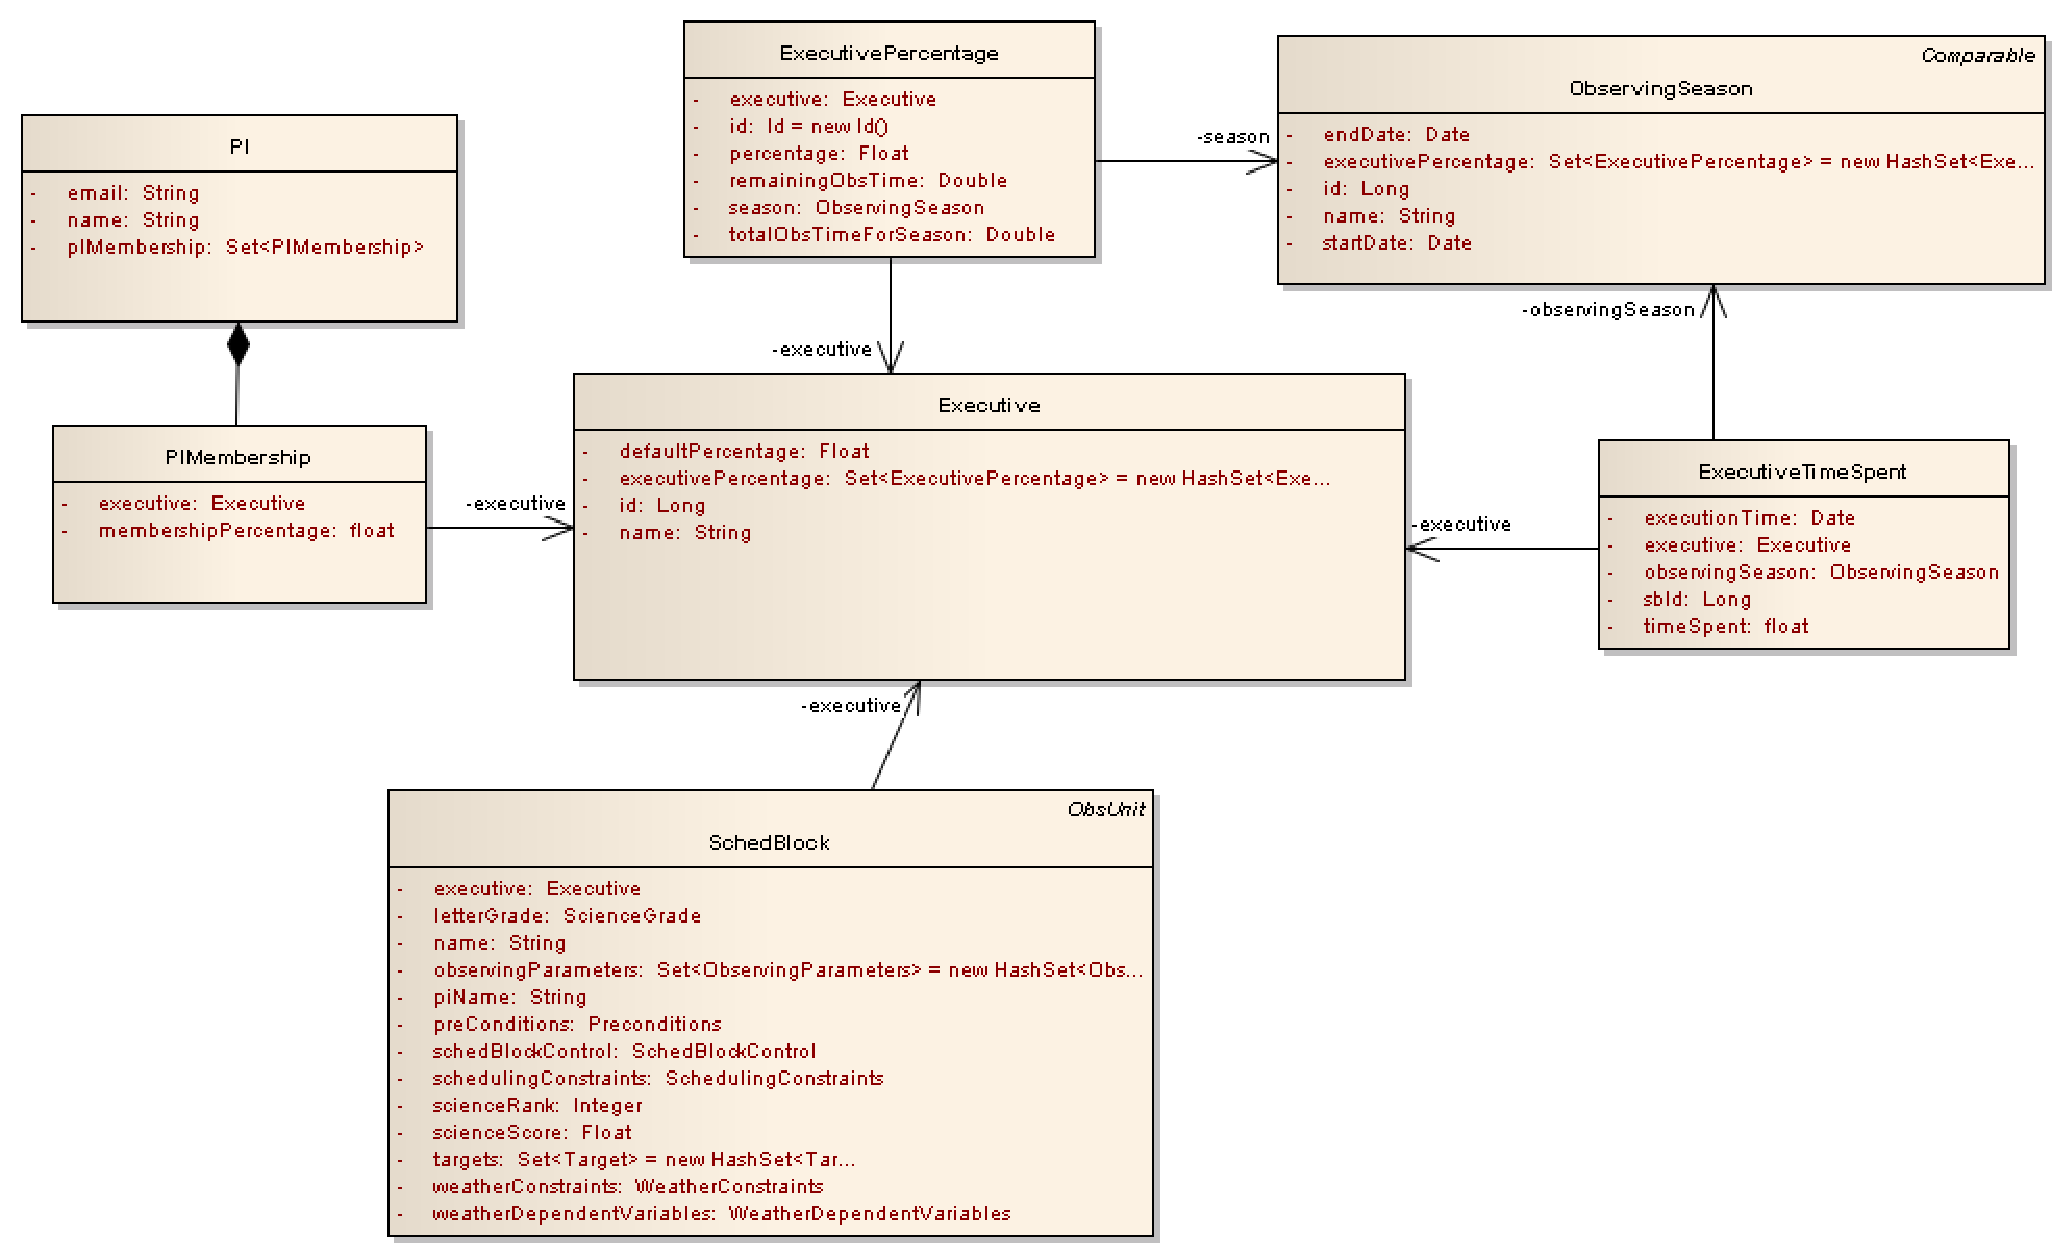
\includegraphics[width=\textwidth]{Executive.pdf}
\caption{Executive data model.}
\label{fig:executivedm}
\end{figure}

The relationship between a SB and an Executive is made though the PI. A PI can be related to more than one
Executive. This relationship is represented in the PIMembership table. For convenience, this relationship
is also maintained directly, as a link between SchedBlock and Executive.

The obsproject package class diagram is shown in Figure~\ref{fig:obsprojectdm}. This package follows closely the APDM
structure, although only the fields that are relevant for the DSA are used. Also, some additional classes
and fields that are not present in the APDM have been added.

\begin{figure}
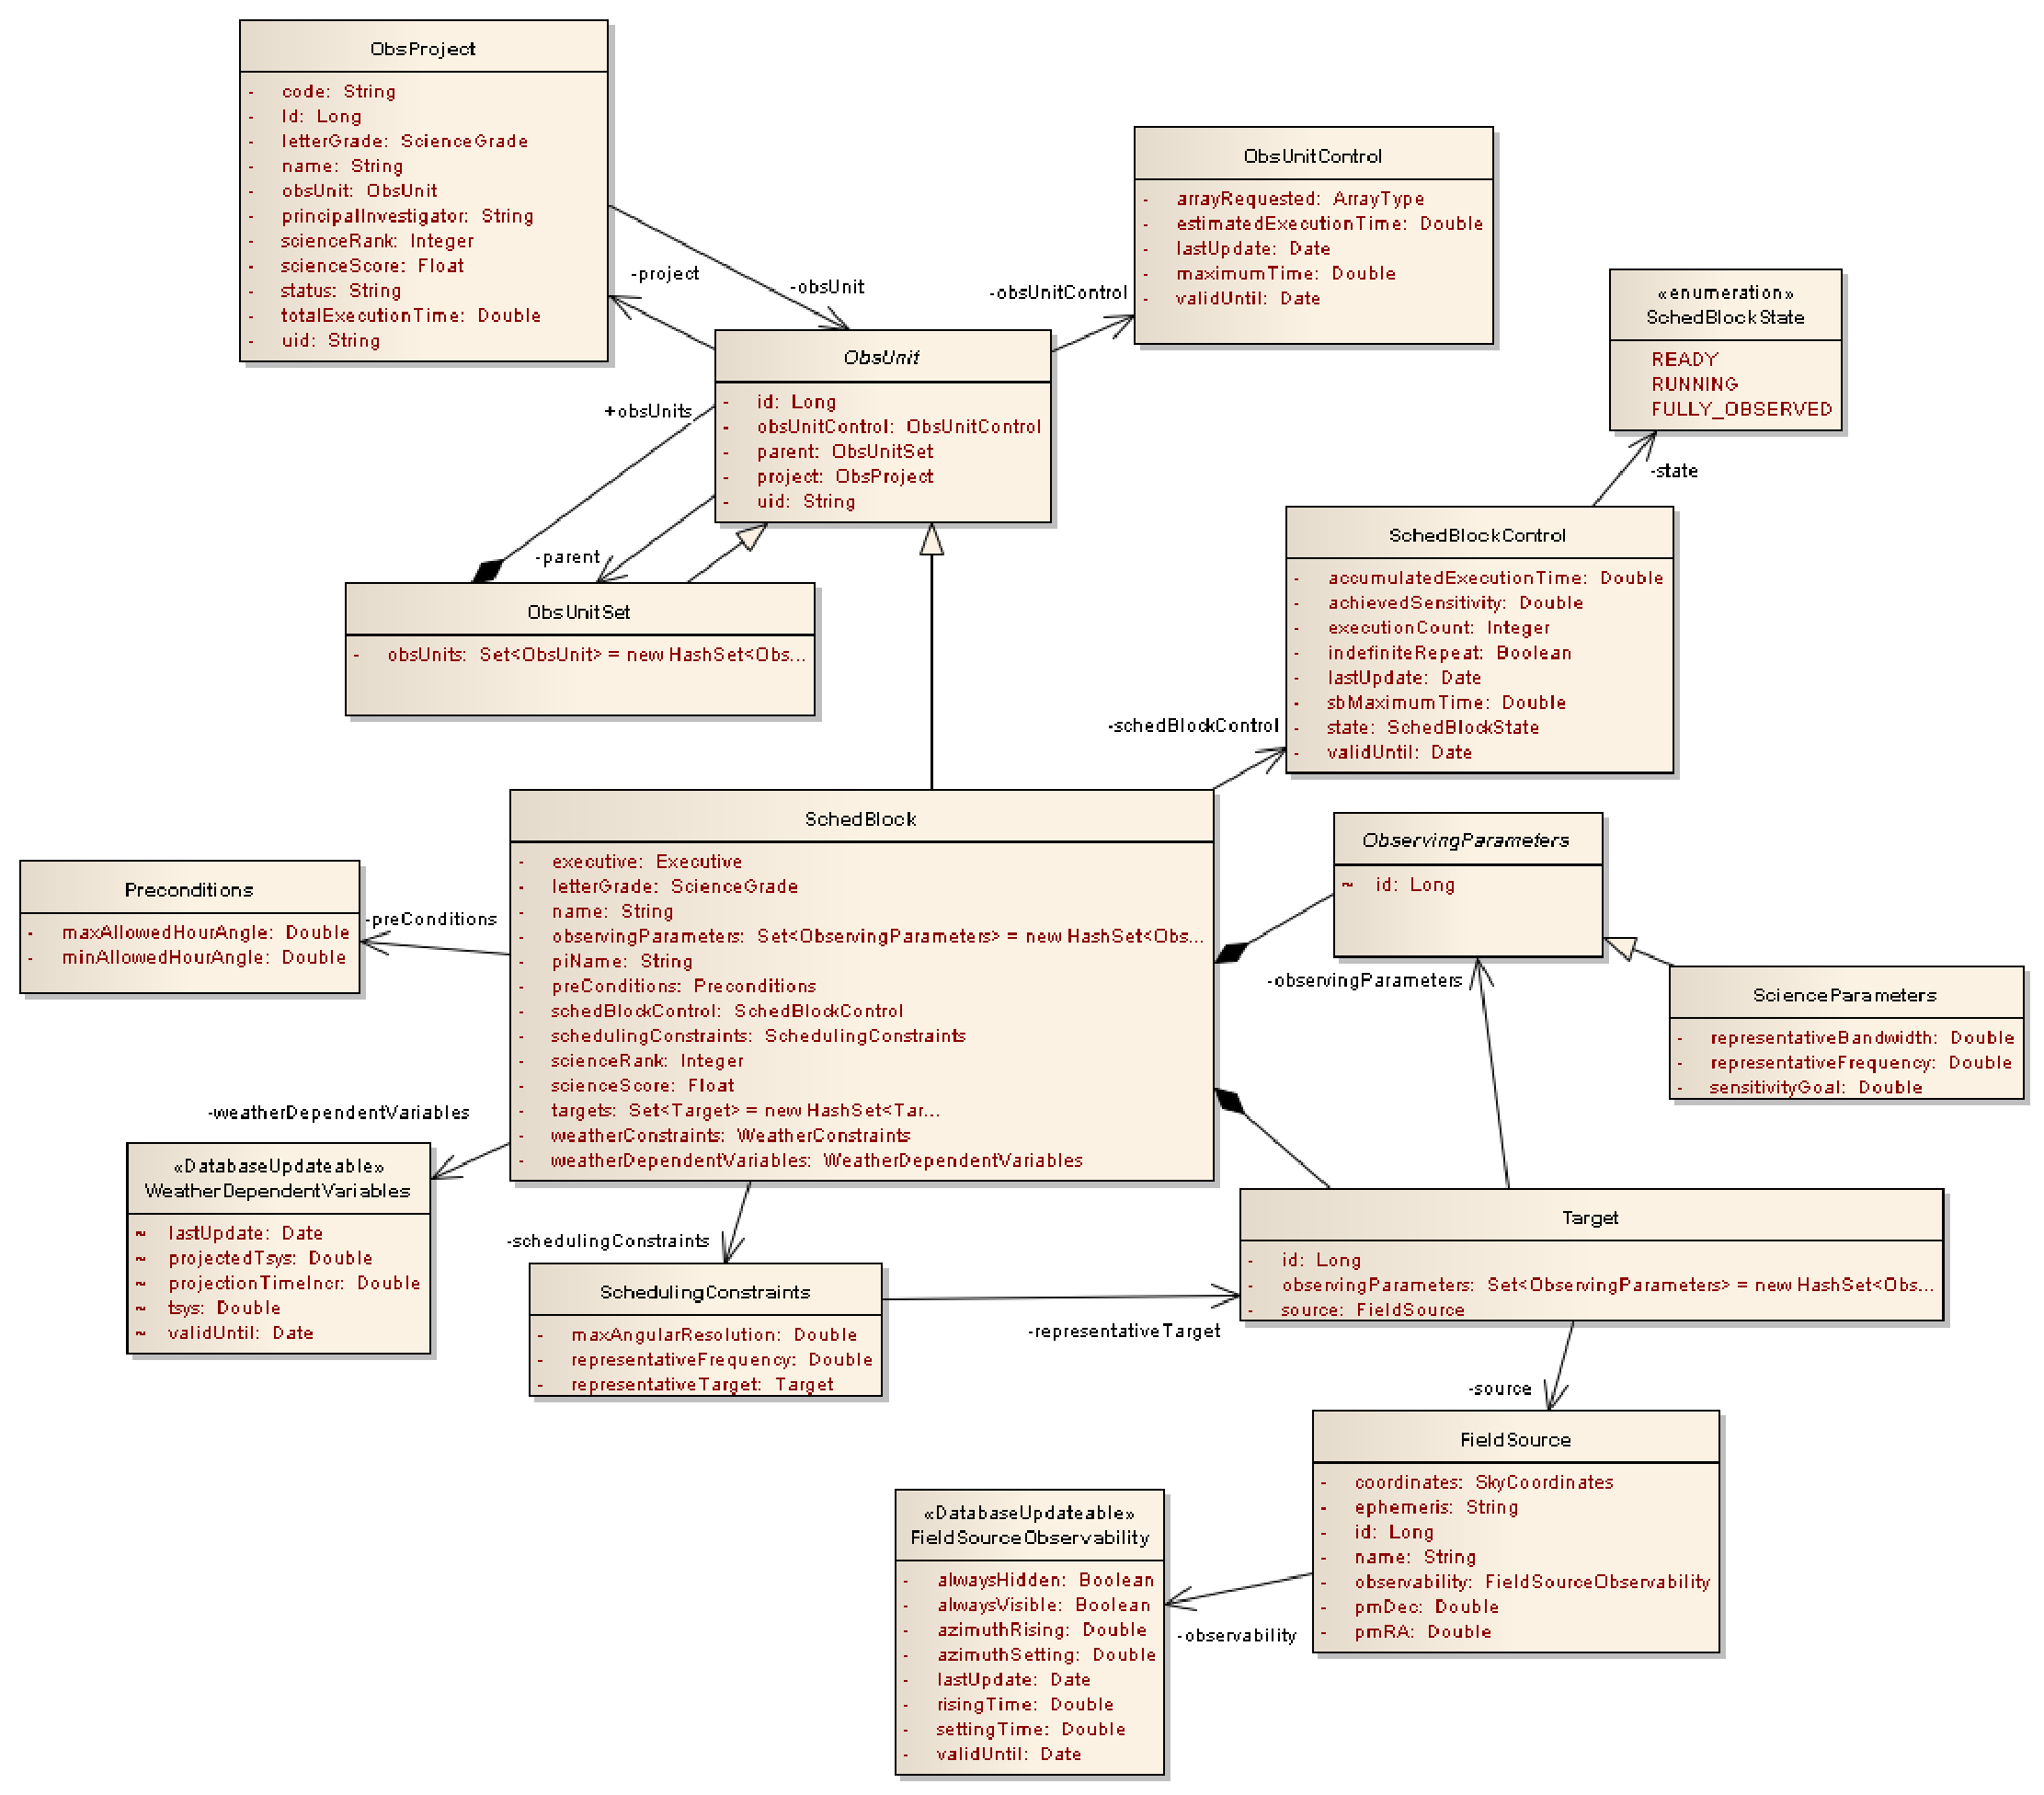
\includegraphics[width=\textwidth]{ObsProject.pdf}
\caption{ObsProject data model.}
\label{fig:obsprojectdm}
\end{figure}

In some cases, the DSA needs to update some of the objects with a certain periodicity. These are marked
as "DatabaseUpdateable". For example, the WeatherDependenVariables class, that contains the Tsys
and projected Tsys, is updated for the relevant SchedBlocks at the beginning of each DSA iteration.
FieldSourceObservability, in the other hand, which contains the LST rising and setting time for a source,
only needs to be updated once, at the beginning of a simulation run.

The observatory package can be seen in Figure~\ref{fig:observatorydm}. This section aims to represent the state of the
telescope hardware throughout the time interval covered by the simulation, including the program of array
configurations.

\begin{figure}
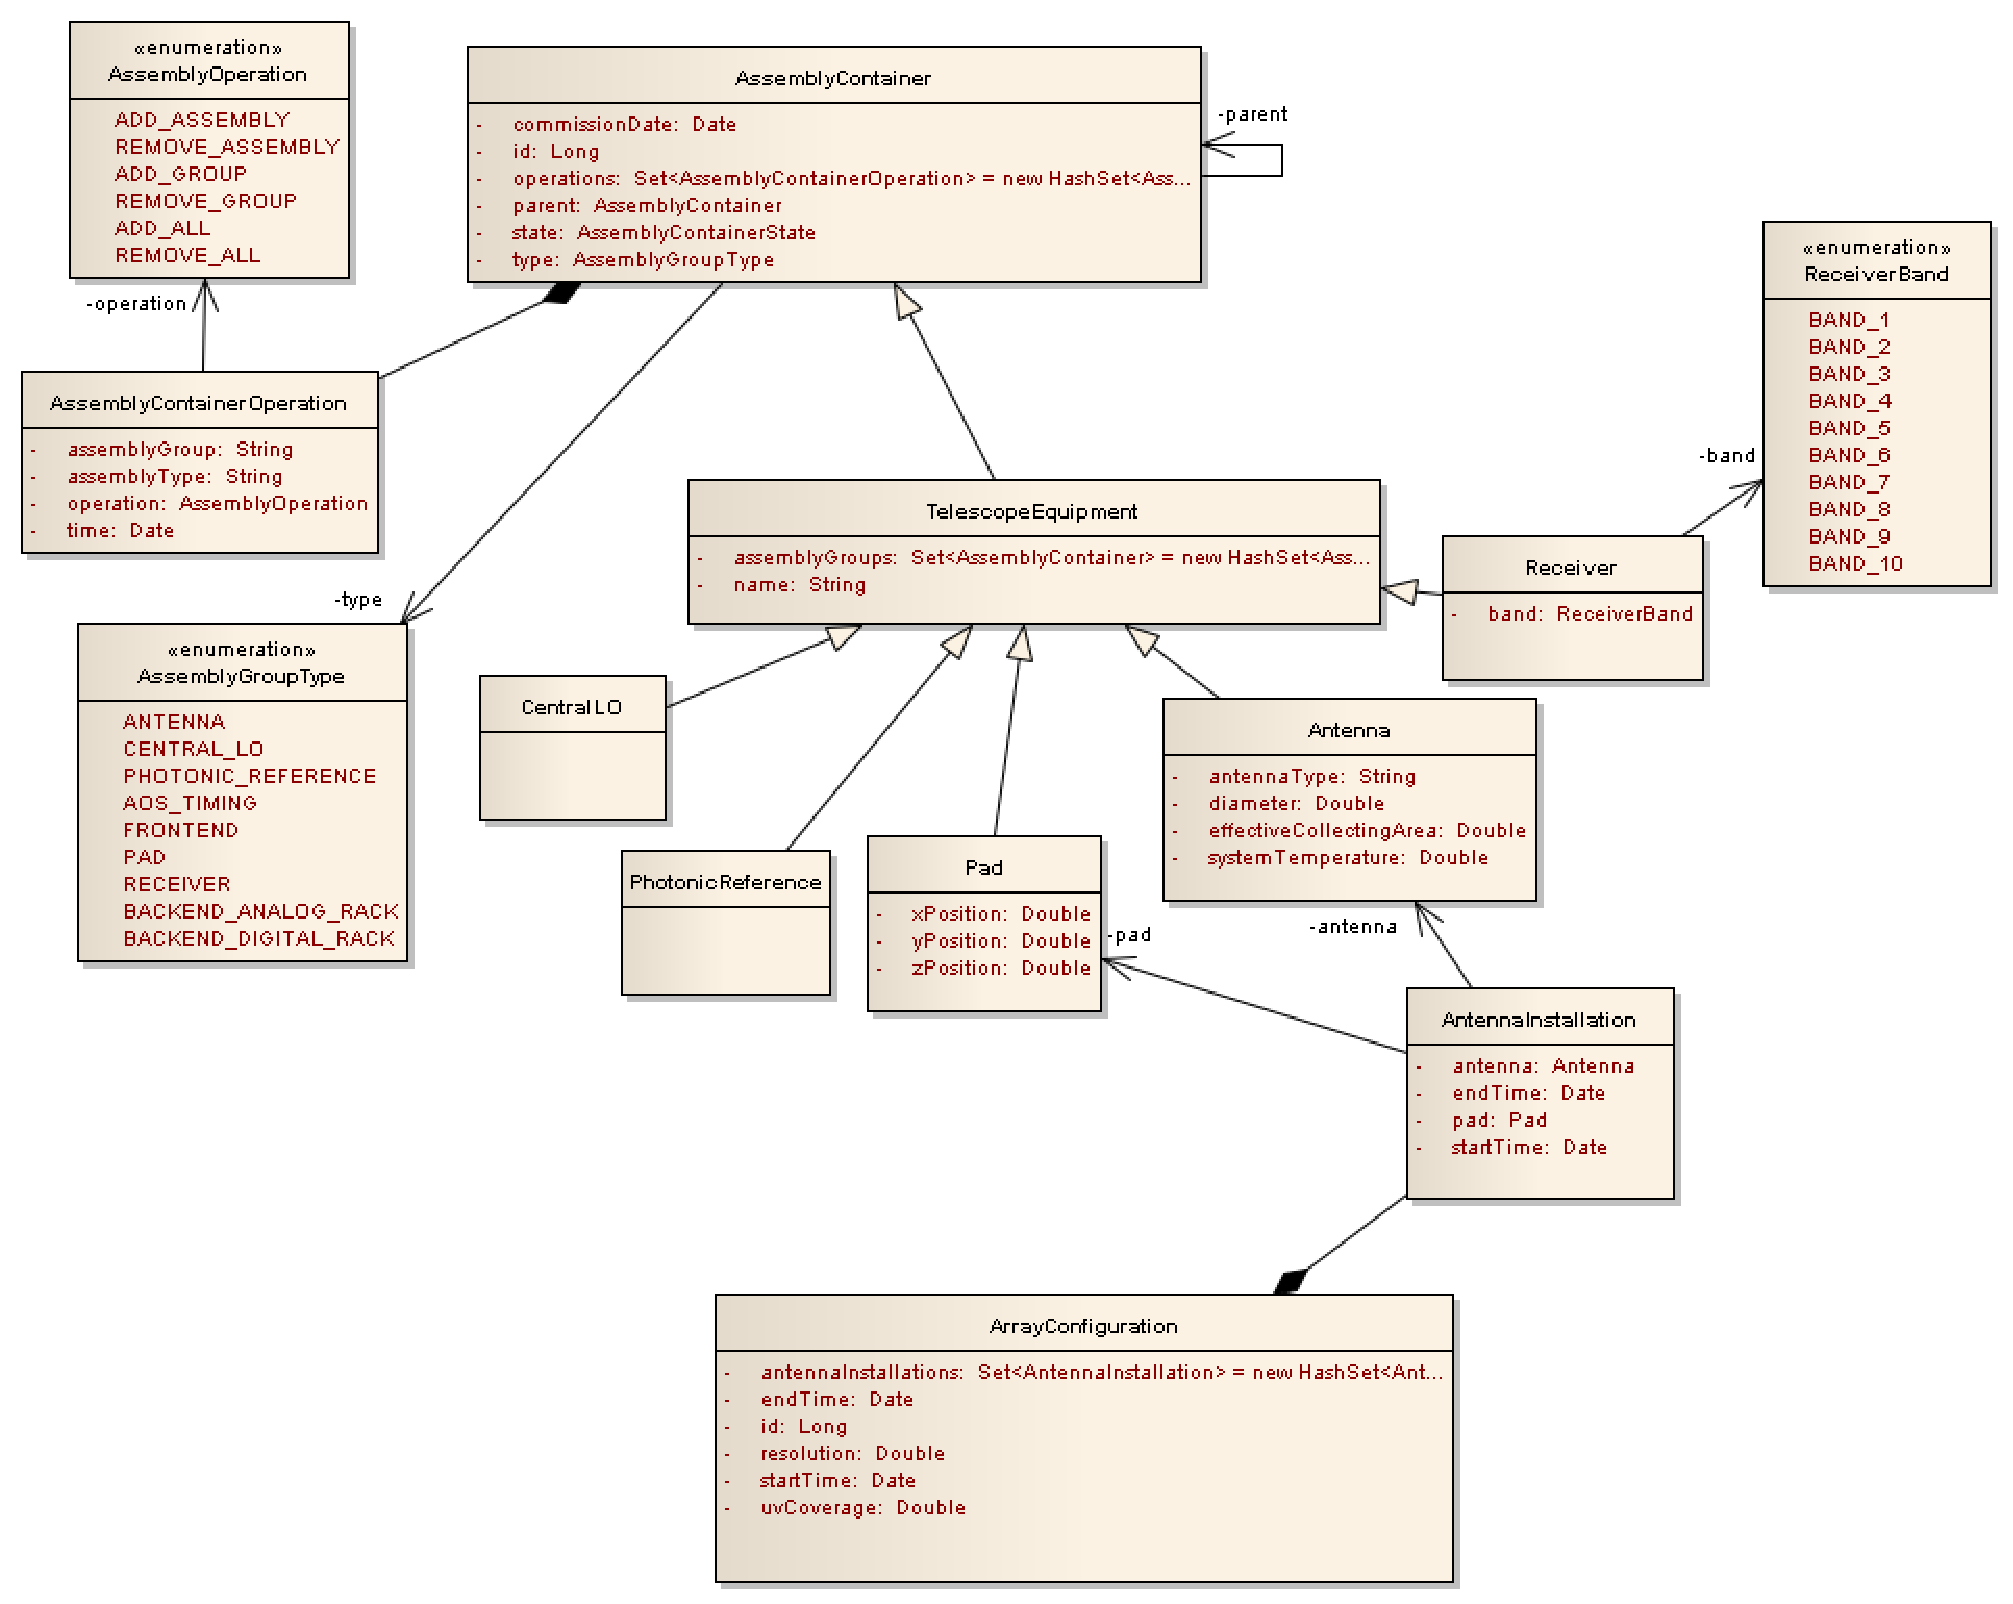
\includegraphics[width=\textwidth]{Observatory.pdf}
\caption{Observatory data model.}
\label{fig:observatorydm}
\end{figure}

The telescope hardware devices are modeled as being either an Assembly, or a TelescopeEquipment, which
can contain other TelescopeEquipment, and/or Assemblies. This hierarchical structure follows the design
of the TMCDB.

Changes in the hardware state are stored as operations over the assemblies or groups of assemblies. The
actual state of the hardware at a given point in time is dealt with following the same design represented
by "DatabaseUpdateable". Records are updated periodically, following the defined operations.
An Antenna and a Pad are linked by AntennaInstallation, a link that is time-dependent. Several
AntennaInstallations conform an ArrayConfiguration. The DSA will start a different scheduler for each
ArrayConfiguration.

The weather section is very simple, and is shown in Figure~\ref{fig:weatherdm}. The atmospheric model table is
maintained as AtmParameters records, and historical weather data is represented as different types of
WeatherHistRecords.

\begin{figure}
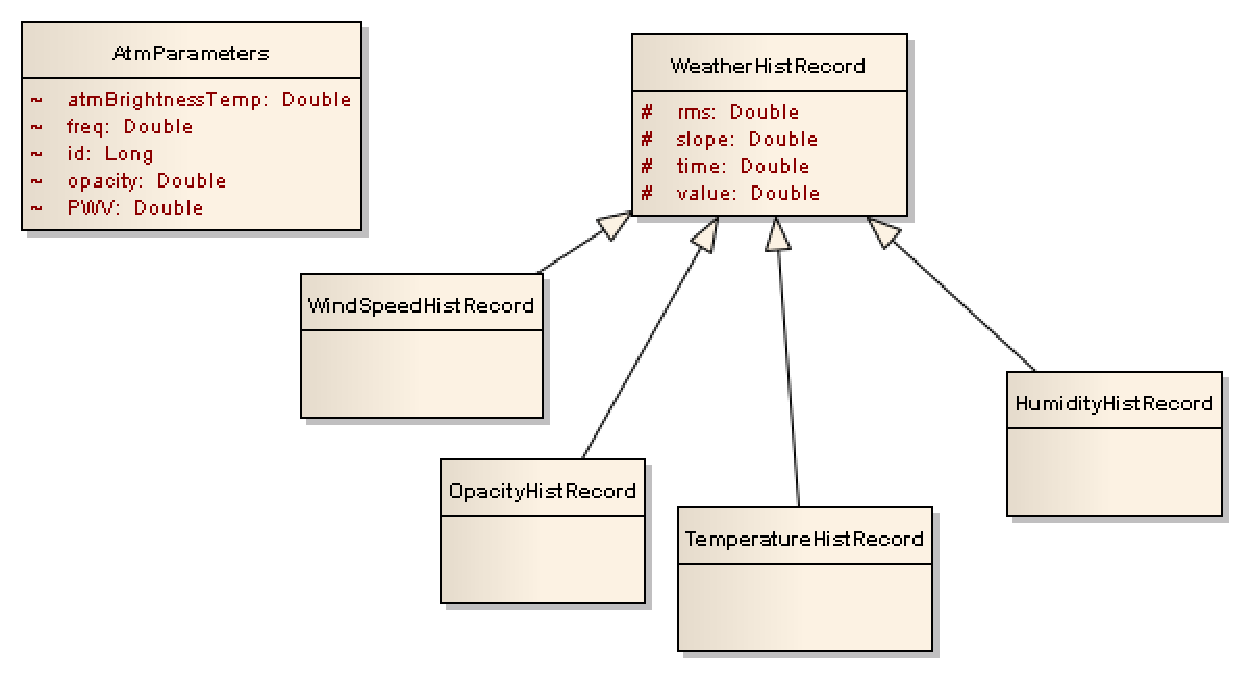
\includegraphics[width=\textwidth]{Weather.pdf}
\caption{Weather data model.}
\label{fig:weatherdm}
\end{figure}

Lastly, Figure~\ref{fig:outputdm}  displays the output package. This package includes classes that represent and summarize
the results of a simulation. Basically, the simulation Results integrate both the Arrays that were created
during the simulation time, and the ObservationProjects that contained SBs that were executed in the
Arrays. SB executions are recorded as SchedBlockResult instances.

\begin{figure}
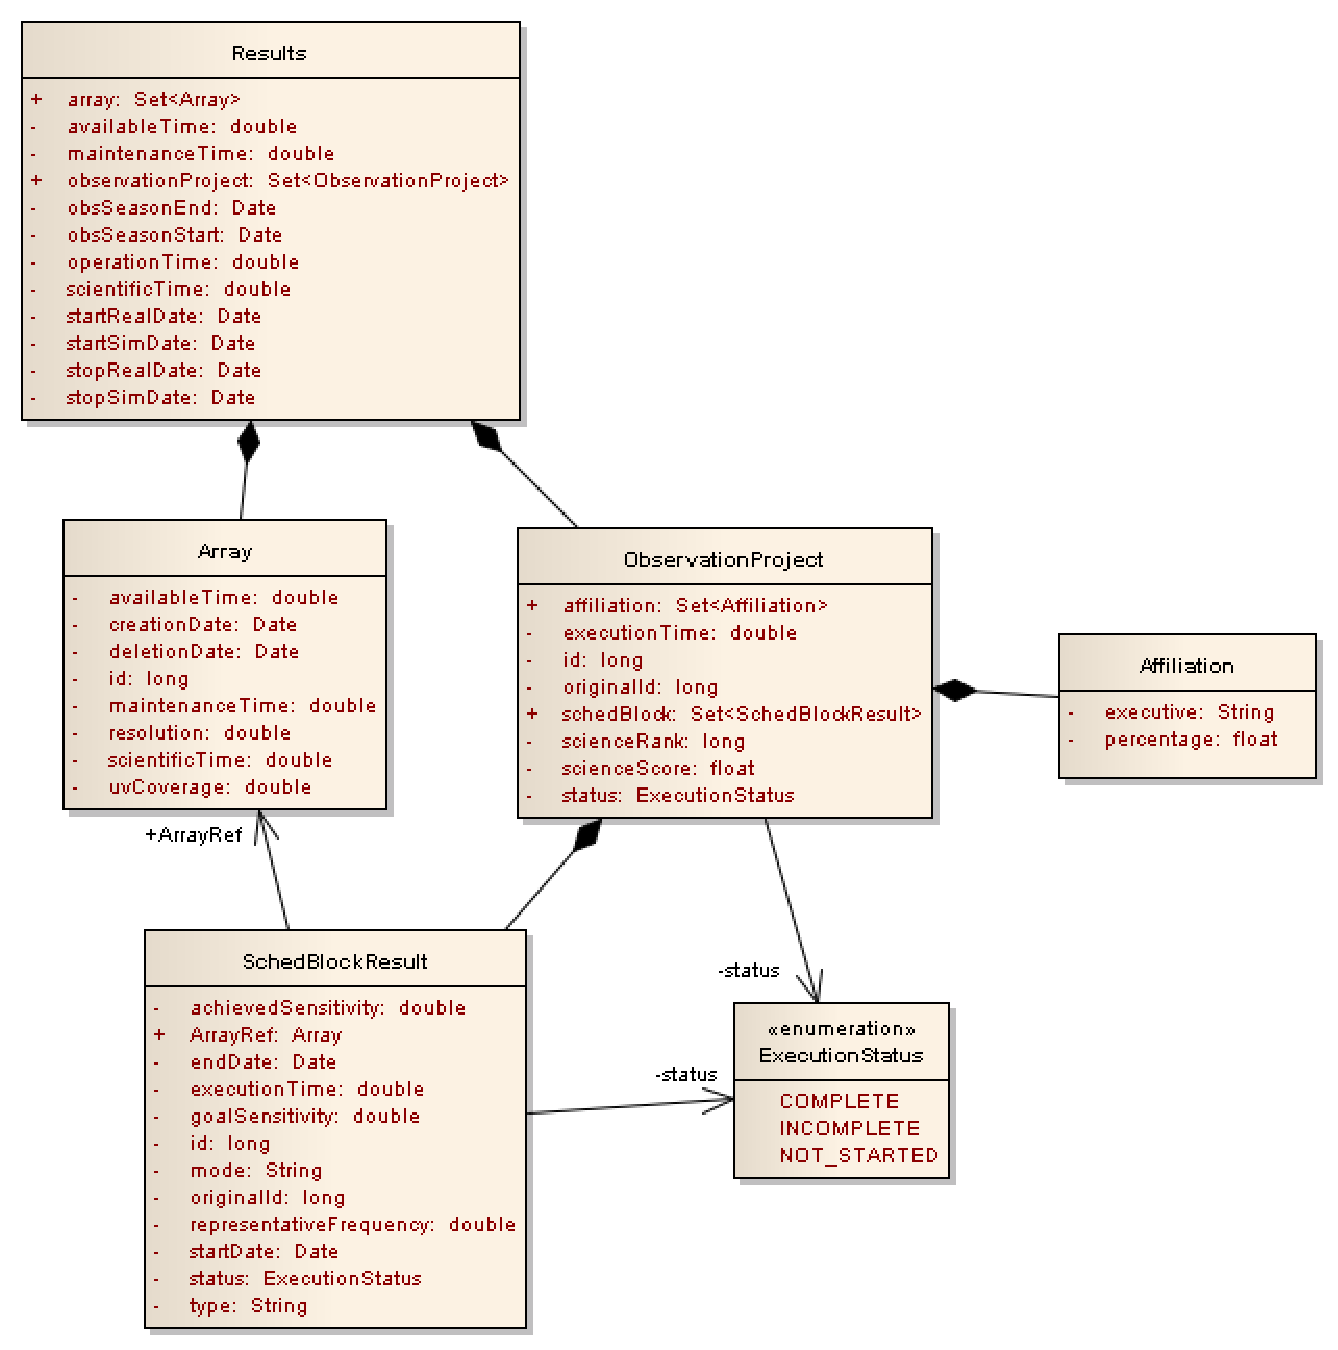
\includegraphics[width=\textwidth]{Output.pdf}
\caption{Output data model.}
\label{fig:outputdm}
\end{figure}

\section{Pre-selection Criterias}

\subsection{Executive remaining time}

Each {\tt SchedBlock} object is associated with an {\tt Executive}. Currently this association is
done through the PI. For each {\tt SchedBlock} there is single {\tt Executive}. It is likely that this
association be modified in the future to account for PIs belonging to many Executives.

Every time that a SB is executed, either a simulated execution or a real execution, the
{\tt ExecutivePercentage.remainingObsTime} field is updated, adding the real observation time,
in the case of a real execution in the telescope; or the {\tt ObsUnitControl.estimatedExecutionTime},
in case the execution is simulated.

The final query for this selector involves several joins. Referring to Figure~\ref{fig:executivedm},
{\tt SchedBlock} is joined with {\tt Executive}, {\tt Executive} with {\tt ExecutivePercentage}, and
{\tt ExecutivePercentage} with {\tt ObservingSeason}. The {\tt ObservingSeason} is contrained to be
the current observing season, and
$$
\mathtt{ObsUnitControl.estimatedExecutionTime}\ \leq \mathtt{ExecutivePercentage.remainingObsTime}.
$$

The required fields in the APDM are:
\begin{itemize}
\item {\tt ObsProject.pI}
\item {\tt SchedBlock.pI}
\item {\tt ObsUnitControl.estimatedExecutionTime}
\end{itemize}

\subsection{Source visibility}

When populating the database, for each {\tt FieldSource} in each {\tt SchedBlock},
a {\tt FieldSourceObservability} object is created (see Figure~\ref{fig:obsprojectdm}).
This class contains the LST of rising and
setting, $LST_r$ and $LST_s$, respectively. These are calculated as:
\begin{eqnarray*}
LST_r & = & 24 - \frac{1}{15} \cos^{-1} (-\tan\phi\tan\delta) + \alpha \\
LST_s & = & \frac{1}{15} \cos^{-1} (-\tan\phi \tan\delta) + \alpha
\end{eqnarray*}
where $\alpha$ is the right ascension, $\delta$ is the declination, and
$\phi$ is the telescope geographical latitude.
This selection operation selects all the SBs for which the current $LST$ falls
between $LST_r$ and $LST_s$, accounting for cases where this range extends to include
the following day.

%
% mountains, etc.
%

The required fields in the APDM are:
\begin{itemize}
\item {\tt SchedBlock.SchedulingConstraints.representativeCoordinates}
\end{itemize}

\subsection{Remaining array time}

The program of array configurations is part of the Observatory database
section (Figure~\ref{fig:observatorydm}). All SBs that comply with the condition:
$$
\mathtt{ObsUnitControl.estimatedExecutionTime} < (\mathtt{ArrayConfiguration.endTime} - t)
$$
where $t$ is the current time, are selected.

The required fields in the APDM are:
\begin{itemize}
\item {\tt ObsUnitControl.estimatedExecutionTime}
\end{itemize}

\subsection{Hour angle restriction}

The purpose of these selection operation is to restrict the SBs selected to
only the ones with representative targets close to the zenith. Given that the observatory
is in the southern hemisphere, a source is close to the zenith when $HA' = HA + 12.0 = LST - \alpha + 12.0$
is small. We express this condition as a quey over the right ascension $\alpha$.

Currently we restrict the $HA$ to be between 8.0 and 16.0 hours.

The required fields in the APDM are:
\begin{itemize}
\item {\tt SchedBlock.SchedulingConstraints.representativeCoordinates}
\item {\tt SchedBlock.Preconditions.minAllowedHA}
\item {\tt SchedBlock.Preconditions.maxAllowedHA}
\end{itemize}

\subsection{Sun avoidance zone}

{\em (To be completed.)}

{\tt SchedBlock.SchedulingConstraints.representativeCoordinates} from the APDM is required.

\subsection{Moon avoidance zone}

{\em (To be completed.)}

{\tt SchedBlock.SchedulingConstraints.representativeCoordinates} from the APDM is required.

\subsection{SB status}

This selector simply filters out all the SBs with state (the state is
kept in {\tt SchedBlockControl.state}) different from {\tt READY}.

The interesting part of this is how the algorithm moves the states
from {\tt READY} to {\tt FULLY\_OBSERVED}. A SB is considered complete
when the achieved sensitivity is equal or less than the sensitivity
goal for the SB.

Currently the algorithm only deals with the case where all the observations
of the same SB are done over the same target, with the same observational
setup (i.e., same correlator configuration and observing frequency). This
is the usual case.

In this case, the RMS noise for multiple observations $\sigma$ is accumulated as
$$
\sigma = \frac{\sqrt{\sum_{i=1}^M \sigma_i^2}}{M}
$$
where $M$ is the number of SBs and $\sigma_i$ is the RMS noise for a single
execution of an SB, calculated differently depending of the type of observation.
For interferometric observations:
$$
\sigma_i^{INT} = \frac{T_{sys}^i}{\eta_Q \sqrt{N_{INT}^i(N_{INT}^i-1)(\Delta\nu)\tau^i}}
$$
where $T_{sys}^i$ is the system temperature, $\eta_Q$ is the correlator sensitivity,
$N_{INT}^i$ is the number of antennas, $\Delta\nu$ is the bandwidth, and $\tau^i$ is
the integration time. All the quantities with the $i$ superscript are specific for the $i$-th
observation.

For single-dish observations
$$
\sigma_i^{SD} = \frac{\alpha T_{sys}^i \sqrt{N_{SD}^i}}{\sqrt{(\Delta\nu)\tau^i}}
$$
where $\alpha$ is a numerical factor that depends on the scanning mode ($\sim 1$ for OTF,
$\sim \sqrt{2}$ for switched observations).

The RMS values are expressed in degrees Kelvin. To convert them to flux units, they are
multiplied by the factor $2k/A_e$ where $k$ is the Boltzmann constant and $A_e$ is the
antenna effective aperture.

These equations don't cover the case of the combined array, where the antennas in the
array have different sizes, nor cover the cases where the bandwidth has been changed
(multi-resolution modes, etc.).

%
% Fudge factor
%

The required fields in the APDM are:
\begin{itemize}
\item {\tt SchedBlock.SchedulingConstraints.representativeCoordinates}
\item {\tt SchedBlock.SchedulingConstraints.representativeFrequency}
\item {\tt SchedBlock.SchedulingConstraints.representativeTarget}. For this target:
\begin{itemize}
\item {\tt ScienceParameters.representativeBandwidth}
\item {\tt ScienceParameters.sensitivityGoal}
\end{itemize}
\item {\tt SchedBlockControl.sBMaximumTime}
\item {\tt ObsUnitControl.maximumTime}
\end{itemize}

\subsection{Array configuration and resolution}

A first order approximation of the resolution that can be attained with a give
array configuration is $\theta = \lambda / l_{max}$ where $l_{max}$ is the maximum
baseline in the array. Each SB defines a range of acceptable resolutions $[\theta_{min}, \theta_{max}]$.
The selection criteria in this case selects all SBs for which
$$
\theta_{min} \leq \frac{\lambda}{l_{max}} \leq \theta_{max}
$$

The required fields from the APDM are:
\begin{itemize}
\item {\tt SchedBlock.SchedulingContraints.representativeFrequency} 
\item {\tt SchedBlock.SchedulingContraints.minAcceptableAngResolution} 
\item {\tt SchedBlock.SchedulingContraints.maxAcceptableAngResolution} 
\end{itemize}

\section{Post-selection Criterias}

\subsection{$T_{sys}$ variation}

The first selection operation that has been implemented tries to ensure that
the weather conditions won't deteriorate significantly during the execution of
an SB. For this purpose, the $Tsys$ calculated using an average of a few data
points taken at the time when the algorithm is executed is compared with the
projected $Tsys$ calculated 30 minutes later (30 minutes being the assumed
average duration of an SB), taking also into consideration the change in elevation
of the SB representative target.

How significant the increase in $Tsys$ needs to be for a SB to be discarded
is under discussion, and in general it will be frequency dependent. In addition
it is possible that some projects decide that non-optimum observing conditions are
fine anyway. For now, an increase in the $Tsys$  of 15-20\% is considered too much
degradation for the SB to be executed.

The calculation of $Tsys$ is done in three steps:
\begin{enumerate}
\item First the Precipitable Water Vapor (PWV) content is determined. There are
several ways of doing this:
\begin{enumerate}
\item Calculate PWV from the Relative Humidity (RH) or the Dew Point. One way
of doing this is found in the MMA Memo No. 237, ``Precipitable Water at the VLA --
1990-1998'', by Bryan Butler. In this paper the PWV is developed as
$$
h = \frac{m_w P_0 H}{\rho_l k T_0}
$$
where $m_w$ is the mass of a water molecule (18 amu), $P_0$ is the water vapor
partial pressure, $H$ is the scale height of water vapor distribution (an
exponential distribution, 1.5 km for the VLA), $\rho_l$ is the density of
liquid water ($\mathrm{gr}/\mathrm{cm}^3$) and $k$ is the Boltzmann constant.

This memo presents a way to estimate $P_0$ from the dew point. In the subsequent
MMA Memo No. 238, ``Precipitable Water at KP -- 1993-1998'', a way of calculating
$P_0$ from the relative humidity is given:
$$
P_0 = 2.409 \times 10^{12} \ RH\ \theta^4 \exp(-22.67\theta)
$$
where $\theta$ is the inverse temperature ($\theta = 300/T_0 $ K), and $RH$ is
the relative humidity.

\item Calculate it from the opacity $\tau_{225}$ at 225 GHz measured by the
tipper. In this case a way of calculating the $PWV$ can be seen in
ALMA Memo 271 ``The Determination of Precipitable Water Vapour at Llano de
Chajnantor from Observations of the 183 GHz Water Line''. $PWV$ can be obtained
by inverting
$$
\tau_{225} = 6.7787\cdot 10^{-3} + 4.0757\cdot 10^{-2} PWV + 9.59\cdot 10^{-4} PVW^2
$$
\item Get the PWV directly from the Water Vapor Radiometers.
\end{enumerate}
When the $PWV$ is available from different sources, the different values
are averaged.

\item Interpolate the ATM tables to determine the opacity $\tau$ and the
atmospheric effective temperature $T_{atm}$. The ATM tables have the following structure:
\begin{eqnarray*}
\tau & = & \tau(\nu_i, PWV_j) \\
T_{atm} & = & T_{atm}(\nu_i, PWV_j)
\end{eqnarray*}
where $\nu_i$ covers the range $20-1000$ GHz with 100 MHz granularity, and $PWV_j$
covers the 7 values 0.4772, 0.658, 0.9134, 1.262, 1.796, 2.748, and 5.186 (mm). 
\item The system temperature is calculated as
$$
T_{sys} = T_{rx} + \eta T_{atm} \left ( 1 - e^{-\tau/\sin(el)} \right ) + (1 - \eta) T_{amb}
$$
where $T_{rx}$ is the receiver temperature, $\eta$ is the forward efficiency (or
feed efficiency, or spillover factor), and $T_{amb}$ is the ambient temperature.

Finally, $Tsys$ is moved to a scale outside the atmosphera:
$$
T_{sys}' = T_{sys} e^{\tau/\sin(el)}
$$
\end{enumerate}

The selection operation filters out all the SBs that don't comply with
$$
\frac{T_{sys}(t+\Delta t) - T_{sys}(t)}{T_{sys}(t)} < 0.15
$$

\subsection{Current $T_{sys}$ selection and scoring}

Besides above criteria, that ensures some degree of weather stability during the execution
of a SB, the algorithm should
favour the SBs that require the most stringent conditions. The stringency of the
required weather conditions can be defined in terms of the opacity and/or $T_{sys}$,
and the phase stability.

Regarding the opacity, a scoring function should be defined to push up SBs with
representative frequency in the higher bands, considering in addition the losses in transparency
in the edges of the bands. In the same way, SBs with representative targets
at low elevations will require better opacity. The exact form of these scoring functions
haven't been defined yet.

A possibility would be to invert the $T_{sys}$ equation for the argument $\tau_\nu/\sin(el)$
(see Figure~\ref{fig:tsyscrit}),
so for a given $T_{sys}^{max}$ the corresponding $x^{max}$ is calculated.
Then the algorithm
\begin{enumerate}
\item Filters out all the SBs for which $\tau_\nu/\sin(el) > x^{max}$.
\item Applies a scoring function that prioritize the SBs with higher
$(\tau_\nu/\sin(el))$. The higher this parameter, the more stringent are 
the weather conditions that the SB require.
\end{enumerate}

\begin{figure}
\includegraphics[width=\textwidth]{tsyscrit.mps}
\caption{$T_{sys}$ based selection and scoring.}
\label{fig:tsyscrit}
\end{figure}


Besides this, it will be necessary to filter out SBs for which the
current phase stability  and wind speed are to bad to observe.
The APDM directly defines requirements for these parameters.

The APDM required fields are:
\begin{itemize}
\item {\tt SchedulingConstraints.representativeFrequency}
\item {\tt SchedulingConstraints.representativeCoordinates}
\item {\tt WeatherConstraints.phaseStability}. {\em Not used yet.}
\item {\tt WeatherConstraints.maxPWVC}. {\em Not used yet.}
\item {\tt WeatherConstraints.maxWindVelocity}. {\em Not used yet.}
\item {\tt WeatherConstraints.seeing}. {\em Not used yet.}
\end{itemize}

\section{Scoring Functions}

The algorithm computes several scoring functions, which are then combined in a
weighted sum. The weight factors are part of the set of parameters that conform
the {\em Scheduling Policy}.

\subsection{Scientific priority score}

Each proposal or project gets assigned a scientific priority, defined by three numbers
$(\mathtt{score},\mathtt{rank},\mathtt{grade})$. The {\tt score} (a float) is assigned by
a specialized commitee (galactic, extra-galactic, etc.). When the proposals that have
been evaluated by different commitees are assembled in one set, there is the possibility
of collisions in the order defined by the {\tt score}. The {\tt rank} (an integer) resolves these
collisions, providing a completely ordered set. On top of this, the {\tt grade} (which can assume
the values A, B, C, or D)

The algorithm computes the scientific priority score as
$$
S = \frac{N_p - (\mathtt{rank} - 1)}{N_p} + K
$$
where $N_p$ is the total number of projects (or proposals), and \\
$$
K = \left\{
    \begin{array}{l l}
    4 & \text{if project grade is $A$} \\
    2 & \text{if project grade is $B$}\\
    1 & \text{if project grade is $C$}\\
    0 & \text{if project grade is $D$}
    \end{array} \right . 
$$

The required fields in the APDM are:
\begin{itemize}
\item {\tt ObsProject.scientificScore} 
\item {\tt ObsProject.scientificRank} 
\item {\tt ObsProject.letterGrade} 
\end{itemize}

\subsection{Hour angle score}

Given that the observatory is located in the southern hemisphere, in order to favor the
SBs that at the current time have their representative source close to the zenith, 
their hour angle should be in the vicinity of 12.0 hours. The hour angle score is
$$
   S = \left\{ \begin{array}{ll}
                0.25\cdot (HA - 12.0) + 1.0 & \text{if $8.0 \leq HA < 12.0$} \\
               -0.25\cdot (HA - 12.0) + 1.0 & \text{if $12.0 \leq HA \leq 16.0$}
               \end{array}
       \right . \
$$

The required fields in the APDM are:
\begin{itemize}
\item {\tt SchedulingContraints.representativeFrequency}
\end{itemize}

\end{document}

